

\begin{comment}
\chapter{Rules for the outer loop}


\subsection{Progress vectors for prerequisites}
\label{sec:preq}

Progress vectors can be used to describe properties of educational components. 
We have small task class with exercises after 
The vector in table \ref{prerequisites.progressvector} describes the prerequisites for our exercise maxi.


\begin{table}[H]
\begin{tabular}{| l | l | r |}
\hline
Key & Progress indicator value\\
\hline
Causal.SimpleExpressionEvaluation & Knowledge\\
Syntax.IFexpression & Knowledge\\
Prelude.GTR & Knowledge\\
Prelude.Plus & Comprehension\\
CS.double& True\\
\hline
\end{tabular}
\caption{Progress vector to define prerequisites.}
\label{prerequisites.progressvector}
\end{table}
 
The student must have read about if an gtr, perhaps because we supplied supportive materials.

We can now easily compare the prerequisites with the student model:
\begin{itemize}
\item $prerequisites \leq studentmodel$
\end{itemize}

Progress vectors may have different content. 
The prerequisites in table  \ref{prerequisites.progressvector} did not specify DomainConcept.Recursion.
Missing attributes in progress vectors are assumed to have a default value of bottom.
In this case it compares as  $(DomainConcept.Recursion \rightarrow Ignorant)$.

\subsection{Progress vectors to update the student model}
\label{sec:pv2sm}
\begin{table}[H]
\begin{tabular}{| l | l | r |}
\hline
Key & Progress indicator value\\
\hline
Syntax.IFexpression & Comprehension\\
Prelude.GTR & Comprehension\\
CD.maxi & True\\
\hline
\end{tabular}
\caption{Progress vector to define objectives.}
\label{objectives.progressvector}
\end{table}

Objectives can also be defined as progress vectors as shown in table \ref{objectives.progressvector}.
We will update the student model after each successful exercises execution.
If it is determined that this exercise was completed successful, then we assert that the student achieved the objectives.
The student model can then be updated by joining the objectives:
\begin{itemize}
\item $ studentmodel_{n+1} = studentmodel_{n} \lor objectives$
\end{itemize}

The updated student model is shown in table \ref{student2.progressvector}.

\begin{table}[H]
\begin{tabular}{| l | l | r |}
\hline
Key & Progress indicator value\\
\hline
DomainConcept.Recursion & Knowledge \\
Causal.SimpleExpressionEvaluation & Application\\
Syntax.IFexpression & Comprehension\\
Prelude.GTR & Comprehension\\
Prelude.Plus & Comprehension\\
RL.expr.plus& 1\\
CS.double& True\\
CD.maxi & True\\
\hline
\end{tabular}
\caption{Update progress vector for overlay student model.}
\label{student2.progressvector}
\end{table}

Like the comparison operation the missing values are assumed to be as bottom. 
 
\subsection{Domain reasoner feedback}
\label{sec:drfeedb}
This section has shown how progress vectors can be used to compare and update a student model.
Current domain reasoners do not yet support progress vectors.
The diagnose function of a domain reasoner might be expanded to support delivering feedback in the form of a progress vector.
We will assume that also properties can be added of student solutions.
Domain reasoners parse the student solution. 
It may be useful to received properties on domain concepts, syntax or prelude functions used.
These properties can be derived from the parse tree .

In the OWL example we have seen that we used counters to keep track of rule execution.

We can also keep track of exercise progress with a progress vector.

To update the exercise progress we introduce an extra operator increment.
An increment is the same as a join, except that counters are added instead of max.

\begin{table}[H]
\begin{tabular}{| l | l | r |}
\hline
Key & Progress indicator value\\
\hline
RL.expr.plus& 5\\
RL.expr.if& 3\\
RL.expr.gtr& 3\\
\hline
\end{tabular}
\caption{Exercise progress: ep1}
\label{exercise1.progress}
\end{table}

\begin{table}[H]
\begin{tabular}{| l | l | r |}
\hline
Key & Progress indicator value\\
\hline
RL.expr.plus& 1\\
finished& True\\
\hline
\end{tabular}
\caption{Domain reasoner diagnose message: diagnose1}
\label{dr1.message}
\end{table}

The tables \ref{exercise1.progress} and \ref{dr1.message} show progress vectors with student progress (ep1) and a
domain reasoner diagnose message as progress vector (diagnose1).

Te model is updated with the the inrement operator.
\begin{itemize}
\item $ep2 = increment \; ep1 \; diagnose1$
\end{itemize}

In table \ref{exercise1.progress} we see the result.

\begin{table}[H]
\begin{tabular}{| l | l | r |}
\hline
Key & Progress indicator value\\
\hline
RL.expr.plus& 6\\
RL.expr.if& 3\\
RL.expr.gtr& 3\\
finished& True\\
\hline
\end{tabular}
\caption{Updated exercise progress: ep2}
\label{exercise1.progress}
\end{table}

Just like the other cases bottom values are substituted for the missing attributes

We cannot determine successful completion with a single comparison operation.


\begin{table}[H]
\begin{tabular}{| l | l | r |}
\hline
Key & Progress indicator value\\
\hline
RL.expr.plus& 1\\
error & True\\
notequivalent & True\\
\hline
\end{tabular}
\caption{Diagnose message with error: diagnose2}
\label{dr.message2}
\end{table}

\begin{table}[H]
\begin{tabular}{| l | l | r |}
\hline
Key & Progress indicator value\\
\hline
RL.expr.plus& 7\\
RL.expr.if& 3\\
RL.expr.gtr& 3\\
finished& True\\
error & True\\
notequivalent & True\\
\hline
\end{tabular}
\caption{Updated exercise progress after error: ep3}
\label{exercise.progress3}
\end{table}

In tables \ref{dr.message2} and \ref{exercise.progress3} we see a diagnose message with an error, and the resulting
exercise progress.
Te model is again updated with the the inrement operator:
\begin{itemize}
\item $ep3 = increment \; ep2 \; diagnose2$
\end{itemize}

If the vector ep3 is greater than the exercise success criteria in table {exercise.crit1}.
However errors are negative. 
The solution is to keep the errors apart.
If the errors are less or equal than bottom (empty progress vector) then we are OK.
To allow some mistakes negative success criteria must be defined.

\begin{table}[H]
\begin{tabular}{| l | l | r |}
\hline
Key & Progress indicator value\\
\hline
RL.expr.plus& 2\\
RL.expr.if& 2\\
RL.expr.gtr& 2\\
\hline
\end{tabular}
\caption{Exercise success criteria crit1}
\label{exercise.crit1}
\end{table}



\subsection{Lightweight reasoning}

We designate the start model as $m_{0}$ and we start with step $s_{1}$.
The steps $s_{1} .. s_{n}$ are the student log.
To update the model we first have increment the model with the step.
Then we must apply rules to the incremented model.
\begin{itemize}
\item $ m_{n+1}' = increment \;m_{n}  \; s_{n+1}  $
\item $ m_{n+1} = apply \; rules \; m_{n+1}' $
\end{itemize}


\subsection{Reasoning about exercise completion}

We have defined rules that determine the outcome of a learning task.
A task has the following state model:

\renewcommand{\figurename}{Figure}

\begin{figure}
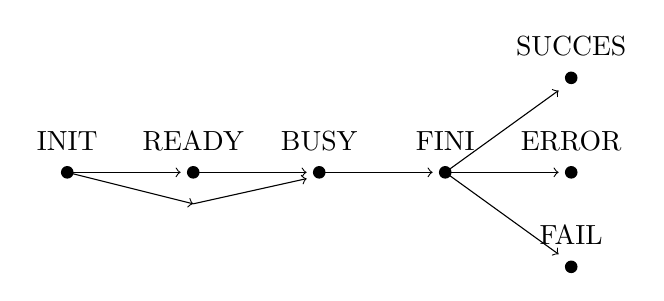
\begin{tikzpicture}[scale=0.08]

\fill[black] (20,20) circle(1);
\node (o3) at (20,25) {INIT};
\fill[black] (40,20) circle(1);
\node (o3) at (40,25) {READY};
\fill[black] (60,20) circle(1);
\node (o3) at (60,25) {BUSY};
\fill[black] (80,20) circle(1);
\node (o3) at (80,25) {FINI};

\fill[black] (100,5) circle(1);
\node (o3) at (100,10) {FAIL};
\fill[black] (100,20) circle(1);
\node (o3) at (100,25) {ERROR};
\fill[black] (100,35) circle(1);
\node (o3) at (100,40) {SUCCES};


\draw [->] (20,20) -- (38,20);
\draw [->] (20,20) -- (40,15);
\draw [->] (40,15) -- (58,19);

\draw [->] (40,20) -- (58,20);
\draw [->] (60,20) -- (78,20);

\draw [->] (80,20) -- (98,7);
\draw [->] (80,20) -- (98,20);
\draw [->] (80,20) -- (98,33);


\end{tikzpicture}
\caption{Learning task state}\label{fig:ltstate}
\end{figure}

The state depicted in figure \ref{fig:ltstate} is derived from multiple Boolean values set by the  diagnose messages from the domain reasoner.
This was outlined in section \ref{sec:atomicpi}. 
The state busy is entered when a create message is received, that sets the created flag.
The state fini is entered when we receive a message with the flag finished.
If the user cancels the exercise the user interface should submit the finished flag.
If the finished flag is set, the state FINI is derived, which is used to trigger rules.
The rules then determine the states SUCCESS, ERROR and FAIL. 
FAIL means the exercise was not finished.


There are three rules to finish the learning task.

%% ODER: format ==         = "\mathrel{==}"
%% ODER: format /=         = "\neq "
%
%
\makeatletter
\@ifundefined{lhs2tex.lhs2tex.sty.read}%
  {\@namedef{lhs2tex.lhs2tex.sty.read}{}%
   \newcommand\SkipToFmtEnd{}%
   \newcommand\EndFmtInput{}%
   \long\def\SkipToFmtEnd#1\EndFmtInput{}%
  }\SkipToFmtEnd

\newcommand\ReadOnlyOnce[1]{\@ifundefined{#1}{\@namedef{#1}{}}\SkipToFmtEnd}
\usepackage{amstext}
\usepackage{amssymb}
\usepackage{stmaryrd}
\DeclareFontFamily{OT1}{cmtex}{}
\DeclareFontShape{OT1}{cmtex}{m}{n}
  {<5><6><7><8>cmtex8
   <9>cmtex9
   <10><10.95><12><14.4><17.28><20.74><24.88>cmtex10}{}
\DeclareFontShape{OT1}{cmtex}{m}{it}
  {<-> ssub * cmtt/m/it}{}
\newcommand{\texfamily}{\fontfamily{cmtex}\selectfont}
\DeclareFontShape{OT1}{cmtt}{bx}{n}
  {<5><6><7><8>cmtt8
   <9>cmbtt9
   <10><10.95><12><14.4><17.28><20.74><24.88>cmbtt10}{}
\DeclareFontShape{OT1}{cmtex}{bx}{n}
  {<-> ssub * cmtt/bx/n}{}
\newcommand{\tex}[1]{\text{\texfamily#1}}	% NEU

\newcommand{\Sp}{\hskip.33334em\relax}


\newcommand{\Conid}[1]{\mathit{#1}}
\newcommand{\Varid}[1]{\mathit{#1}}
\newcommand{\anonymous}{\kern0.06em \vbox{\hrule\@width.5em}}
\newcommand{\plus}{\mathbin{+\!\!\!+}}
\newcommand{\bind}{\mathbin{>\!\!\!>\mkern-6.7mu=}}
\newcommand{\rbind}{\mathbin{=\mkern-6.7mu<\!\!\!<}}% suggested by Neil Mitchell
\newcommand{\sequ}{\mathbin{>\!\!\!>}}
\renewcommand{\leq}{\leqslant}
\renewcommand{\geq}{\geqslant}
\usepackage{polytable}

%mathindent has to be defined
\@ifundefined{mathindent}%
  {\newdimen\mathindent\mathindent\leftmargini}%
  {}%

\def\resethooks{%
  \global\let\SaveRestoreHook\empty
  \global\let\ColumnHook\empty}
\newcommand*{\savecolumns}[1][default]%
  {\g@addto@macro\SaveRestoreHook{\savecolumns[#1]}}
\newcommand*{\restorecolumns}[1][default]%
  {\g@addto@macro\SaveRestoreHook{\restorecolumns[#1]}}
\newcommand*{\aligncolumn}[2]%
  {\g@addto@macro\ColumnHook{\column{#1}{#2}}}

\resethooks

\newcommand{\onelinecommentchars}{\quad-{}- }
\newcommand{\commentbeginchars}{\enskip\{-}
\newcommand{\commentendchars}{-\}\enskip}

\newcommand{\visiblecomments}{%
  \let\onelinecomment=\onelinecommentchars
  \let\commentbegin=\commentbeginchars
  \let\commentend=\commentendchars}

\newcommand{\invisiblecomments}{%
  \let\onelinecomment=\empty
  \let\commentbegin=\empty
  \let\commentend=\empty}

\visiblecomments

\newlength{\blanklineskip}
\setlength{\blanklineskip}{0.66084ex}

\newcommand{\hsindent}[1]{\quad}% default is fixed indentation
\let\hspre\empty
\let\hspost\empty
\newcommand{\NB}{\textbf{NB}}
\newcommand{\Todo}[1]{$\langle$\textbf{To do:}~#1$\rangle$}

\EndFmtInput
\makeatother
%

\begin{listing}
\begingroup\par\noindent\advance\leftskip\mathindent\(
\begin{pboxed}\SaveRestoreHook
\column{B}{@{}>{\hspre}l<{\hspost}@{}}%
\column{5}{@{}>{\hspre}l<{\hspost}@{}}%
\column{E}{@{}>{\hspre}l<{\hspost}@{}}%
\>[B]{}\Varid{learningTaskErrorRule}\mathbin{::}\Conid{Rule}{}\<[E]%
\\
\>[B]{}\Varid{learningTaskErrorRule}\mathrel{=}{}\<[E]%
\\
\>[B]{}\hsindent{5}{}\<[5]%
\>[5]{}[\mskip1.5mu \Varid{learningTaskState}\;\Conid{FINI},\Varid{learningTaskHasErrors}\mskip1.5mu]{}\<[E]%
\\
\>[B]{}\hsindent{5}{}\<[5]%
\>[5]{}\mathbin{=->}{}\<[E]%
\\
\>[B]{}\hsindent{5}{}\<[5]%
\>[5]{}[\mskip1.5mu \Varid{taskInError}\mskip1.5mu]{}\<[E]%
\\[\blanklineskip]%
\>[B]{}\Varid{learningTaskSuccessRule}\mathbin{::}\Conid{Rule}{}\<[E]%
\\
\>[B]{}\Varid{learningTaskSuccessRule}\mathrel{=}{}\<[E]%
\\
\>[B]{}\hsindent{5}{}\<[5]%
\>[5]{}[\mskip1.5mu \Varid{learningTaskState}\;\Conid{FINI},\Varid{learningTaskSucces},\Varid{objectivesMet}\mskip1.5mu]{}\<[E]%
\\
\>[B]{}\hsindent{5}{}\<[5]%
\>[5]{}\mathbin{=->}{}\<[E]%
\\
\>[B]{}\hsindent{5}{}\<[5]%
\>[5]{}[\mskip1.5mu \Varid{taskSuccess},\Varid{updateStudentModel}\mskip1.5mu]{}\<[E]%
\\[\blanklineskip]%
\>[B]{}\Varid{abandonedRule}\mathbin{::}\Conid{Rule}{}\<[E]%
\\
\>[B]{}\Varid{abandonedRule}\mathrel{=}{}\<[E]%
\\
\>[B]{}\hsindent{5}{}\<[5]%
\>[5]{}[\mskip1.5mu \Varid{learningTaskState}\;\Conid{FINI},\Varid{learningTaskSucces},\Varid{notP}\;\Varid{objectivesMet}\mskip1.5mu]{}\<[E]%
\\
\>[B]{}\hsindent{5}{}\<[5]%
\>[5]{}\mathbin{=->}{}\<[E]%
\\
\>[B]{}\hsindent{5}{}\<[5]%
\>[5]{}[\mskip1.5mu \Varid{taskFailed}\mskip1.5mu]{}\<[E]%
\\[\blanklineskip]%
\>[B]{}\Varid{readyRule}\mathbin{::}\Conid{Rule}{}\<[E]%
\\
\>[B]{}\Varid{readyRule}\mathrel{=}{}\<[E]%
\\
\>[B]{}\hsindent{5}{}\<[5]%
\>[5]{}[\mskip1.5mu \Varid{learningTaskState}\;\Conid{INIT},\Varid{prerequisitesMet}\mskip1.5mu]{}\<[E]%
\\
\>[B]{}\hsindent{5}{}\<[5]%
\>[5]{}\mathbin{=->}{}\<[E]%
\\
\>[B]{}\hsindent{5}{}\<[5]%
\>[5]{}[\mskip1.5mu \Varid{taskReady}\mskip1.5mu]{}\<[E]%
\ColumnHook
\end{pboxed}
\)\par\noindent\endgroup\resethooks
\caption{The rules for learning task finishing}\label{fig:ltFiniRules}
\end{listing}



Listing \ref{fig:ltFiniRules} shows the rules for finishing the learning taks and updating the student model.
It is small Domain Specific Language (DSL) where standardized predicates and actions are combined into rules.
The operator =-\textgreater creates a rule.
We have created the following predicates and actions:
\begin{itemize}
\item learningTaskState \textless state\textgreater: True if the learning task argument is in the given state.
\item learningTaskSucces : Tests if the domain reasoner returned any errors.
\item learningTaskHasErrors: Negation of learningTaskSucces
\item objectivesMet : Tests if the completion criteria are complete as outlined in section \ref{sec:drfeedb}.
\item prerequisitesMet: Test if the student has met the prerequisites for the exercises.
\item notP : an operator to negate the predicate.
\item askSuccess, taskFailed, askInError, taskReady: actions that return a model with the taskclass and learningtask with one flag set.
The vectors contain no other attributes.
\item updateStudentModel, an action that copies the objectives vector from the learning task to the student model as described in \ref{sec:pv2sm}.

\end{itemize}

The rules are mutually exclusive, the predicates exclude each other, but cover every possible substate when the learning task is in state FINI.
They are idempotent. 
The state that they test on is updated. 
This prevents them from firing again for this task.
The last property is not very important, as the output would be absorbed if fired twice.

These rules can be used for many exercises that have fixed objectives.
For exercises where multiple solutions are possible a more refined rule is needed.
In the length exercise we see that there are multiple solutions. 
Each solution provides evidence for certain domain concepts, but it may depend on the choosen solution.
In that case a solution would be to have the domain reasoner report back which extra objectives have been met.
These can be joined with predefined objectives and then the rules above can be applied.

We see that the learning task metadata bridges a gap between domain reasoner rules and domain concepts.
There is no single rule that proves that the student can evaluate simple expressions.
In this task class we have enough variability, so that we may assume that the student understands simple expression evaluations.
It cannot take this conclusion from individual domain reasoner diagnose actions or rule firings.

\section{Task selection, based on prerequisites}
VanLehn has written an article in which he describes the outer loop and four choices for learning task selection \citep{vanlehn2006}.
One of them is called mastery learning, based on a theory (also by Bloom) called mastery learning.
If we translate this to the TenSteps and our reasoner, then this is easy to implement.
When the student needs to select the next task, we present the learning tasks from the current task class, for which he meets the prerequisites.

We have seen that the task state diagram in figure \ref{fig:ltstate} that there is a task state READY.
This state is assigned by the readyRule (listing \ref{fig:ltFiniRules}).
The predicate prerequisitesMet tests the prerequisites as outlined in section \ref{sec:preq}.

We can use the query from this rule to select the tasks that we rank highest in our recommendation to the student.
It is up to other system components, such as the user interface to enforce such rules or give the student complete freedom.

In this example task class on expression evaluation we can guide the student through the curriculum.
We have defined properties CSdouble, CSmaxi and CScombined.
We want the student to start with exercises of type double, then maxi and then a combined exercise, which is the most complicated.

We can set for example CSmaxi as objective for exercises of type maxi and as prerequisite for exercises of type combined.
It is easy to select exercises where we meet the prerequisites, yet have not achieved the objectives with the comparison operators we have defined.
When an exercise maxi is finished the combined exercises appear immediately as the highest ranked.

We can get this to work in a completely declarative way.
All that the course author has to do is carefully analyse the variations in exercises and define objectives, completion criteria and prerequisites.


\end{comment}

 
 













 



 




